\documentclass[pdftex,12pt,a4paper]{article}
\pdfpagewidth 8.5in
\pdfpageheight 11.6in
\linespread{1.3}
\usepackage{anysize}
\marginsize{2.5cm}{2.5cm}{2.5cm}{2.5cm}

\usepackage[utf8]{inputenc}
\usepackage[T1]{fontenc}
%\usepackage[magyar]{babel}
\usepackage{indentfirst}
\usepackage{amsmath}
\usepackage{subcaption}
\usepackage{float}
\usepackage{graphicx}
\usepackage{braket}
\usepackage{tensor}
\usepackage{hyperref}

%\usepackage{listings}

\DeclareMathOperator{\Ai}{Ai}
\DeclareMathOperator{\Bi}{Bi}
\DeclareMathOperator{\Aip}{Ai^\prime}
\DeclareMathOperator{\Bip}{Bi^\prime}
\DeclareMathOperator{\Ti}{Ti}
\DeclareMathOperator{\ctg}{ctg}
\DeclareMathOperator{\sgn}{sgn}
%\DeclareMathOperator{\max}{max}
\let\Im\relax
\DeclareMathOperator{\Im}{Im}
\DeclareMathOperator{\Tr}{Tr}
\newcommand{\op}[1]{\hat{#1}}
\newcommand{\norm}[1]{\left\lVert #1 \right\rVert}
\newcommand*\Laplace{\mathop{}\!\mathbin\bigtriangleup}

\newcommand{\aeqref}[1]{\az{\eqref{#1}}}
\newcommand{\Aeqref}[1]{\Az{\eqref{#1}}}

%---------------------------------------------------------------------------------------------------------------------
\usepackage{fancyvrb,newverbs,xcolor}

\definecolor{cverbbg}{gray}{0.93}

\newenvironment{cverbatim}
 {\SaveVerbatim{cverb}}
 {\endSaveVerbatim
  \flushleft\fboxrule=0pt\fboxsep=.5em
  \colorbox{cverbbg}{\BUseVerbatim{cverb}}%
  \endflushleft
}
\newenvironment{lcverbatim}
 {\SaveVerbatim{cverb}}
 {\endSaveVerbatim
  \flushleft\fboxrule=0pt\fboxsep=.5em
  \colorbox{cverbbg}{%
    \makebox[\dimexpr\linewidth-2\fboxsep][l]{\BUseVerbatim{cverb}}%
  }
  \endflushleft
}

\newcommand{\ctexttt}[1]{\colorbox{cverbbg}{\texttt{#1}}}
\newverbcommand{\cverb}
  {\setbox\verbbox\hbox\bgroup}
  {\egroup\colorbox{cverbbg}{\box\verbbox}}
%---------------------------------------------------------------------------------------------------------------------
%\frenchspacing
\begin{document}

	\centerline{\bf\LARGE Comparing linear PDE solvers}\vskip0.4truein
	\centerline{\LARGE Computer simulations in physics}\vskip0.4truein
	\centerline{\Large\sc Kürti Zoltán}\vskip0.10truein
	%\centerline{\includegraphics[scale=0.5]{./elte_cimer_color.pdf}}
	\vskip0.4truein
	\centerline{\Large{\today}}
	\thispagestyle{empty}
	\newpage
	\tableofcontents
	\newpage
	\section{Introduction}
		Based on feedback about the last project, in this project I will be more focused on explaining my thought processes and motivations. I will also use more informal language as it is better suited to describe the journey I took while working with partial differential equations.
	\subsection{Motivation}
		The importance of numerically solving partial differential equations can hardly be overstated both in purely academic and engineering fields. At the same time I also like working on both partial and ordinary differential equations, this was one of the reasons my first project involved differential equations too. I dream about obtaining solutions for complicated situations in general relativity, but that's simply not feasible during a couple weeks, in fact I'm not even sure a single person could get meaningful results in this field. So I have to set realistic goals and the obvious first step is to start with a simple linear problem, like the heat equation.
		
		I also like to implement everything on my own, and I also like to come up with my own ideas even if I'm no the first to do so. This method takes a long time and generally isn't optimized for obtaining a result fast and with the less amount of energy. During evaluating a lab measurement to write the report or during a BSc. thesis the focus is on getting results in physics, not programming, and time is critical. In these situations usually people can't afford to begin the project by writing for loops, multiplications and additions in C, I certainly couldn't. This course however does focus on computer programming and writing low level algorithms. All in all this is the perfect opportunity for me to spend time on solving the heat equation on my own.
	\section{Solution outline}
		The first problem I thought about was calculating the laplacian on a discretized grid. This seemed to be an important and frequent operation while solving linear partial differential equations. While working on this problem I created the \ctexttt{coefficients.py} file. This file contains functions that help finding coefficients to approximate the laplacian at a point based on neighboring points up to different orders and with different conditions on the error terms. The functions generally work in $N$ dimensions, although the time for computations often grows exponentially with the number of dimensions. Some of the methods work for irregular grids, which would be very useful in case the discretization of a problem was matched to the geometry of the problem. I did not investigate this aspect, but it is a high priority extension I would make if I continue this project. With these functions it is possible to reproduce all the results about stencils in \cite{patra}, but my approach applies to irregular and also higher dimensional cases.
		
		The next step was to test some of these stencils I got from \ctexttt{coefficients.py}. I focused on one and two dimensional cases and compared single and double precision calculations too. Solving partial differential equations isn't just about choosing the right algorithms. A huge part of the process is finding optimal hyperparameters for the algorithm, like the resolution of discretization, the time step, relaxation parameters, precision of the floating point operations and so on. The choice of these parameters makes or breaks the success of the calculation. My impression so far is that there is no general rule for finding an optimal value for a parameter directly. Experimentation is needed, and this experimentation process can be sped up dramatically by good intuition. This part of the project certainly helped me to make more informed guesses during these types of experimentation.
		
		The last component to solve the first concrete problem is treating boundary conditions. My goal was to be able to handle arbitrary geometries both with Dirichlet and Neumann type boundary conditions. I did meat this goal in two dimensions and my solution generalizes to higher dimensions easily (adding one or two more nested for cycles depending on the function in question). The basic idea applies to irregular discretization, although in that case additional data structures would be needed to look up nearby points. To demonstrate this capability I solved the heat equation in a circle using a square grid for discretization with different combinations of Dirichlet and Neumann boundary conditions. \cite{gaussian,conduction}
	\section{Floating point precision}
		The speed of algorithms is critical for these problems. Especially as the dimension of the problem grows, discretization can quickly lead to millions of points, which need to be updated each time step. in a naiiv implementation calculating the laplacian on a grid is cache constrained. This is because each neighboring points only used a couple times (depending on the size of the stencil) before the calculation moves on and the element is replaced in the cache with other elements. Later in the next row this original value will have to be loaded again, if the rows are long enough. In my computer the L1 cache is $32kiB$. This is enough to hold $4096$ double precision floating point number. Using a 5x5 stencil for the laplacian to calculate each row the program has to load 5 rows of the original data, and the results of the calculation go to the L1 cache first too. Depending on the cache update policy even with a couple hundred elements long row elements may need to be loaded multiple times.
		
		This can be reduced by changing the order in which the laplacian is calculated. Instead of calculating it row by row, for large grids it may be more efficient to calculate the result in square chunks, designed to align with cache lanes ($64B$ on my computer) while maximizing the area of it with the constraint that it fits into the cache. This method would increase the number of uses a single value after each load and so would decrease the total amount of cache operations.
		
		Another great improvement could be the usage of single precision numbers. The discretization of the differential equation already introduces an error that can easily be bigger than single precision. Therefore to store the results of a calculation it ia probably enough to use single precision floating point numbers. The problem comes when the change of the solution is slow compared to the grid resolution (which is a desirable property if we want to minimize the error caused by discretization). The difference of two close floating point numbers will have a large error as the significant digits cancel out. This works against minimizing the discretization error. Increasing the precision of the number representation or using higher order approximations for the laplacian with smaller resolution may be two options to improve this situation.
	\subsection{Precision, step size and error order}
		In one dimension the laplacion of $f$ can be calculated as
		\begin{equation}
			\Laplace f_i = \frac{f_{i+1} - 2f_i + f_{i-1}}{h^2} + \mathcal{O}(h^4)
			\label{1laplace4}
		\end{equation}
		and as
		\begin{equation}
			\Laplace f_i = \frac{-\frac{1}{12}f_{i+2} + \frac{4}{3}f_{i+1} - \frac{5}{2}f_i + \frac{4}{3}f_{i-1} - \frac{1}{12}f_{i-2}}{h^2} + \mathcal{O}(h^6).
			\label{1laplace6}
		\end{equation}
		These expressions can be obtained from the taylor expansion of $f$ around $x_i$, this method will be discussed later more generally. In the first test program I calculated the laplacian of the sine function for different resolutions using equations \ref{1laplace4}. and \ref{1laplace6} both with single and double precision. The results are summarized in figure \ref{1dpdf}, the plot was made using the \texttt{1d.py} file and the data to be plotted was generated with the \texttt{1d64-32laplace} executable. The error on the figure is the biggest difference between the discretized laplacian and the analytic formula. The region on which the calculation was carried out is $2\pi$ long, and $N$ represents the number of points of the discretized grid.
		\begin{figure}[H]
			\centering
			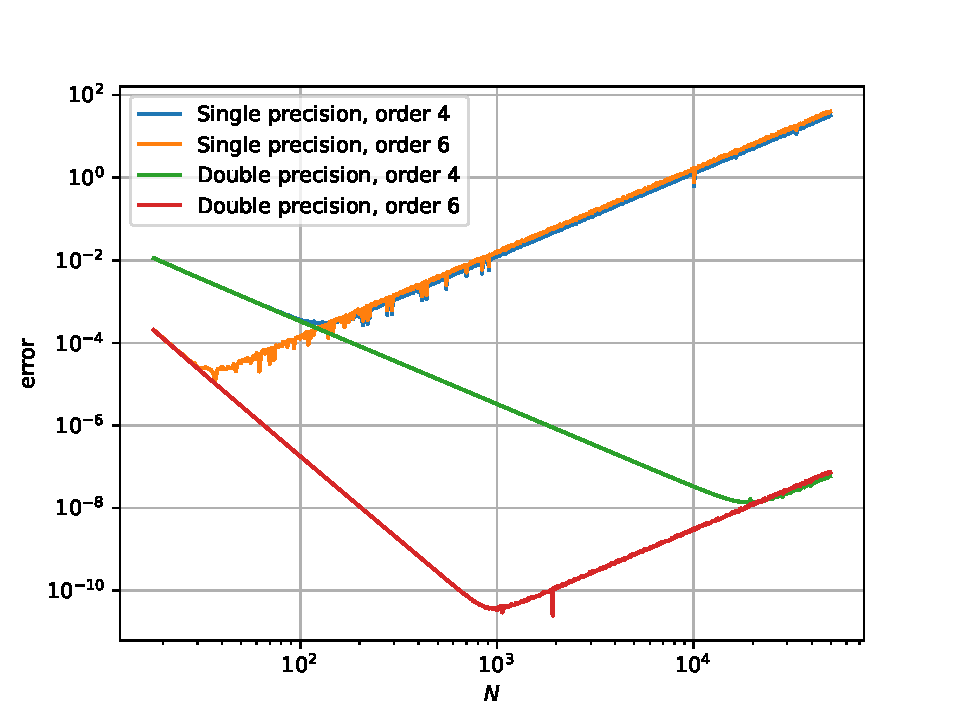
\includegraphics[scale=1]{./figs/1d.pdf}
			\caption{Error values of the discrete laplace for approximation with 4th and 6th order errors and single and double precision. }
			\label{1dpdf}
		\end{figure}
		It can be seen that there are two sources of error. One is the discretization error that decreases as $\frac{1}{N^4}$ or $\frac{1}{N^6}$. The other is the error coming from rounding error when two almost equal floating point numbers are subtracted. The key takeaway is that there is an optimum in precision, neither too big nor too small grid distances work. I observed similar behavior for two dimensional stencils as will be discussed later, and I expect the same for higher dimensions.
	\section{Higher order in many dimensions}
		Based on the above simple one dimensional case study, and as can be expected without any experiments, the most precise way to obtain the laplacian on a grid is using high precision floating point numbers and a finite difference approximation with higher order error terms. Obtaining the coefficients of these stencils becomes a non trivial task, and in the following section I will discuss my solution to this problem.
	\subsection{Designing the kernels}
		The code I will discuss can be found in the \texttt{coefficients.py} file. 
	\subsection{Testing the kernels}
		
	\section{Boundary conditions, where numeric methods shine}
		
	\section{Conclusion}
		
	\bibliographystyle{abeld}
    \bibliography{ref}
\end{document}








